\section{РАСЧЕТЫ И СООБРАЖЕНИЯ ПО КУХОННОМУ ХОЗЯЙСТВУ ДЛЯ ПРАВИЛЬНОГО РАСПРЕДЕЛЕНИЯ КУПЛЕННЫХ ИЛИ ЗАГОТОВЛЕННЫХ ПРИПАСОВ}% отдел 1

Обязанности хозяйки следующие: 
\begin{enumerate}
	\item запасать провизию, закупать ее лично или надзирать, чтобы закупаемые припасы были наилучшего качества и соответствующей цены;
	\item выдавать провизию, сколько чего потребно, для изготовление обеда, завтрака и проч. из назначенных кушаньев;
	\item распределять кушанья, т.~е. назначать из каких блюд должен состоять обед, завтрак и ужин;
	\item надзирать, чтобы все кушанья приготовлялись по правилам поваренного искусства;
	\item наблюдать за чистотою и экономиею в хозяйстве, чтобы все изготовлялось опрятно, безвредно для здоровья семьи и с тем вместе было бы сопряжено с возможно меньшими расходами.
\end{enumerate}

Но для выполнения этих обязанностей необходимо: 
\begin{enumerate}
	\item понимать толк в различных предметах провизии, уметь безошибочно определять их качество, отличать от подмесей и знать цены на них в различное время года; 
	\item знать точно и верно развес; 
	\item быть вполне знакомою с изготовлением различных кушаньев, зная определительно, сколько чего на то или другое из них потребно;
	\item уметь распоряжаться как можно выгоднее данною провизиею, т.~е. чтобы ничто не пропадало даром, например, взяв кусок говядины фунтов в семь, вырезать лучшую часть на жаркое и, если выйдет, на фрикадельки, а кости обратить на суп в дополнение к бульону из супового куска мяса и~т.~д.
\end{enumerate}

Весьма понятно, что это очень трудно не только для молодой, только что начавшей жить своим домом, женщины, но даже и для более опытной, уже занимающейся несколько лет кухнею, хозяйки. Из этого ясно, как необходимо для всякой хозяйки иметь под рукою книгу, которою она могла бы руководствоваться во всех вышесказанных случаях.

Одно из главнейших оснований экономии в хозяйстве, без сомнения,~--- запас провизии. Как бы мало хозяйство это ни было, все-таки необходимо иметь под рукою те припасы, которые входят в состав большей части кушаньев и вместе с тем легко сохраняются, не подвергаясь скоро порче. Так, необходимо запасать в соответственном количестве: муку, масло, крупу, но было бы крайне неблагоразумно закупать для маленького хозяйства по нескольку десятков фунтов мяса, и~т.~д. Закупка удобных к сбережению и употребительнейших в хозяйстве припасов гуртом имеет две выгоды: 1) что, закупаемые в большом количестве, они обходятся дешевле, и вместе с тем всегда есть возможность приобрести их самого лучшего качества, и 2) что, имея под рукою необходимые припасы, хозяйки избавлены от излишних мелочных хлопот. Купите, например, четверку лаврового листа,~--- она в лавке стоит 10 коп. сер., и если у вас семья из пяти или шести человек, то ее хватит вам месяца на два; купите же той же приправы копейки на две или на три, и вам ее едва хватит на два кушанья.

Для большего удобства помещаем тут реестр припасов, которые необходимо иметь всегда дома, предоставляя расчислить стоимость их по той таблице с ценами съестных припасов в Петербурге, какая помещена в предпоследнем отделе этой книги, именно в XXIII.

Для семейства в 4–-6 человек\footnote{Для семейства из 10, 15 человек нужно запасать вдвое и втрое более.}.

\noindentМуки крупичатой не менее 10 фун.\\
Муки заправочной не менее 4 фун.\\
Муки картофельной не менее 3 фун.\\
Крупы гречневой крупной не менее 5 фун.\\
Крупы гречневой средней не менее 5 фун.\\
Крупы ячневой не менее 3 фун.\\
Крупы пшеничной не менее 4 фун.\\
Крупы овсяной не менее 3 фун.\\
Крупы перловой не менее 3 фун.\\
Крупы манной не менее 6 фун.\\
Крупы смоленской не менее 4 фун.\\
Рису не менее 5 фун.\\
Саго простого не менее 3 фун.\\
Саго тапиоку не менее 2 фун.\\
Масла чухонского столового или т.~н. мызного не менее 10 фун.\\
Масла русского\footnote{Русское масло употребляется только для жаренья жарких, блинов и проч. Его очень хорошо можно заменять говяжьим жиром. Для этого нужно покупать говяжий жир (от 10–-15 коп. сер. за фунт), топить его на легком огне и затем, слив, дать застыть и сохранять в холодном месте.} не менее 10 фун.\\
Сушеного белого гороху не менее 5 фун.\\
Сушеного зеленого гороху не менее 5 фун.\\
Белой фасоли не менее 4 фун.\\
Чечевицы не менее 3 фун.\\
Картофелю 3.5 четверика или куль.\\
Соли крупной для кушанья не менее 10 фун.\\
Соли мелкой для стола не менее 5 фун.\\
Русского перцу не менее 0.5 фун.\\
Английского перцу не менее 0.5 фун.\\
Лаврового листу не менее 0.5 фун.\\
Кардамону не менее 1/8 фун.\\
Корицы не менее 1/8 фун.\\
Гвоздики не менее 1/8 фун.\\
Мускатного ореха не менее 1/8 фун.\\
Мускатного цвета не менее 1/8 фун.\\
Сладкого миндалю не менее 2 фун.\\
Горького миндалю не менее 0.5 фун.\\
Изюму не менее 5 фун.\\
Кишмишу не менее 5 фун.\\
Коринки не менее 5 фун.\\
Черносливу не менее 3 фун.\\
Макарон обыкновен. толстых не менее 5 фун.\\
Макарон полутолстых не менее 4 фун.\\
Макарон итальянских не менее 3 фун.\\
Вермишели не менее 3 фун.\\
Яиц не менее 100 штук.\\
Сахару не менее 0.5 пуда.\\
Белого сахарного песку бастеру не менее 0.5 пуда.\\
Сарептской горчицы не менее 1 фун.\\

Вот главные припасы, которые необходимо иметь дома в каждом, хотя и самом малом хозяйстве. Выгода от таких запасов очевидная и не требует объяснения. Держать все это, особенно в таком малом количестве, как здесь показано в вышеприведенном реестре, весьма легко, так как для этого не требуется особого помещения, а просто шкаф с отделениями и ящиками, который можно поставить в прохладное место. Для семейств же больших, которые делают запасы в большом количестве, на зиму, необходимы: ледник, погреб и кладовая, о которых будет сказано ниже, в конце этой книги.

Чтобы хозяйка не теряла лишнего времени при выдаче провизии, необходимо держать, смотря по величине хозяйства, в кладовой или шкафу, все на своем месте. Мука и крупы должны сохраняться в деревянных банках; изюм, перец, мелкий сахар и проч.~--- в выдвижных ящиках и банках; некоторые же предметы можно держать просто в картузах, как они куплены. Притом необходимо наклеить на каждый картуз, ящик или банку надпись, чтобы не нужно было рыться при выдаче провизии. Масло, русское и чухонское, по мнению некоторых хозяек, сохранять всего удобнее следующим образом: развесив его полуфунтами, скатать из каждого полуфунта шарик. При выдаче давать один, два или три шарика, смотря по тому, требуется ли полфунта, фунт или полтора фунта того или другого масла. Мызное или столовое масло сохраняется или подобным же образом, или же в кадушках, и в таком случае его выдают ложками.

Для выдачи провизии хозяйкам следует иметь в кладовой:

Во-первых, столовую серебряную ложку.

Во-вторых, медный или жестяной гарнц.

В-третьих, обыкновенный стакан средней величины. Таких стаканов в одной большой бутылке из-под шампанского, т.~е. в одну четверть гарнца, три; в штофе, т.~е. в полгарнце~--- шесть, следовательно, в одном гарнце~--- двенадцать.

Вторым важным предметом в хозяйстве служит точное знание развеса провизии. Так как при выдаче этой последней было бы слишком затруднительно руководствоваться весами или мерою, т.~е. взвешивать или отмеривать мерою каждую вещь, которая может потребоваться для того или другого кушанья, и притом иногда в слишком незначительном количестве, то прилагаем тут реестр веса разных главных припасов, определяя его по возможности ложками и стаканами, что нам кажется всего удобнее и проще:

\noindent1 фунт крупичатой муки равняется 3 стакан.\\
1 ложка крупичатой муки равняется 1/3 стакан.\\
1 фунт картофельной муки равняется 2.5 стакан.\\
1 фунт гречневой муки равняется 2.5 стакан.\\
1 фунт гречневой крупной крупы равняется 2 1/8 стакан.\\
1 фунт гречневой средней мелкой равняется 2 1/6 стакан.\\
1 фунт гречневой средней мелкой равняется 2 1/4 стакан.\\
1 фунт смоленской крупы равняется 2.5 стакан.\\
1 фунт перловой крупы полуголандки равняется 2 1/8 стакан.\\
1 фунт перловой крупы голандки равняется 2 1/4 стакан.\\
1 фунт ячневой крупы равняется 2 1/3 стакан.\\
1 фунт рису равняется 2 стакан.\\
1 фунт манной крупы равняется 2.5 стакан.\\
1 фунт пшеничной крупы равняется 2 1/8 стакан.\\
1 фунт саго равняется 2 1/3 стакан.\\
1 фунт овсяной крупы равняется 2 3/4 стакан.\\
1 фунт русского масла равняется 2 стакан. или 8.5 ложек.\\
1 фунт чухонского масла равняется 2 стакан. или 8.5 ложек.\\
1 фунт растопленного масла равняется 1 3/4 стакан.\\
1 фунт сахару кусками равняется 3 3/4 стакан. или 32 кускам.\\
1 фунт мелкого сахару равняется 1 7/8 стакан.\\
1 фунт сахарного песку равняется 2.5 стакан.\\
1 столовая ложка мелкого сахару ровно с краями равняется 1 лоту.\\
16 мелко истолченных сухарей равняется 1 стакан.\\
0.5 тертой французской булки равняется 1 стакан.\\
1 фунт белой французской булки равняется 2.5 булки.\\
1 фунт черствой французской булки равняется 2 3/4 булки.\\
1 фунт мелко изломанной вермишели равняется 4.5 стакан.\\
1 фунт сметаны равняется 1 2/3 стакан.\\
1 фунт жареного молотого кофе равняется 5 стакан. легко насыпанным.\\
4 плитки шоколаду равняется 1 фунту.\\
1 фунт мелко истолченного шоколаду равняется 2 стакан.\\
1 фунт русского перцу в зернах равняется 3 стакан.\\
1 фунт английского перцу в зернах равняется 3 стакан.\\
1 фунт мелко истолченного перцу равняется 2 1/3 стакан.\\
1 фунт лаврового листу равняется 1.5 гарнца.\\
1 фунт горчицы равняется 2 2/3 стакан.\\
1 фунт соли крупной равняется 2 1/3 стакан.\\
1 фунт соли мелкой равняется 2 стакан.\\
1 фунт белого гороху равняется 2 1/8 стакан.\\
1 фунт белой фасоли равняется 2 1/3 стакан.\\
1 фунт чечевицы равняется 2 1/8 стакан.\\
1 фунт сушеного мелкого зеленого горошку равняется 2 2/3 стакан.\\
1 фунт изюму равняется 3 1/4 стакан.\\
1 фунт кишмишу равняется 3 стакан.\\
1 фунт коринки равняется 3 стакан.\\
1 фунт миндалю равняется 3 стакан.\\
1 фунт черносливу равняется 2 1/3 стакан.\\
1 фунт очищенной смородины равняется 2 1/4 стакан.\\
1 фунт вишен, клубники, малины и пр. равняется 3 стакан.\\
1 фунт клюквы равняется 2 стакан.\\
1 фунт варенья равняется 1.5 стакан.\\
Маленький мускатный орех равняется 0.5 золотн.\\
Чайная ложка мелко истолченной корицы равняется 0.5 золотн.\\
60 штук кардамону равняется 1 золотн.\\
70 штук гвоздики равняется 1 золотн.\\
0.5 вершка ванили равняется 1 золотн.\\
1 пластинка желатину или телячьего клею равняется 1 золотн.\\

В дополнение к расчетам, определяющим меру и вес различных съестных припасов, находим полезным приложить, при сем, тот общий вывод, какой выработан, по этому предмету, многолетнею практикой.

Для провизии сухой как то: муки, крупы, сухих бобов, гороха, мелкого сахару, свежих и сухих ягод, и проч.\\
1 фунт равняется 2 стакан. или 16 стол. ложк. или 64 чайн. ложк.\\
0.5 фун. равняется 1 стакан. или 8 стол. ложк. или 32 чайн. ложк.\\
1/4 фун. равняется 0.5 стакан. или 4 стол. ложк. или 16 чайн. ложк.\\
1/8 фун. равняется 1/4 стакан. или 2 стол. ложк. или 8 чайн. ложк.\\
6 золотн. равняется 0 стакан. или 1 стол. ложк. или 4 чайн. ложк.\\
3 золотн. равняется 0 стакан. или 0.5 стол. ложк. или 2 чайн. ложк.\\

Для масла нетопленого и сахарного варенья\\
1 фунт равняется 1.5 стакан. или 8 стол. ложк. или 24 чайн. ложк.\\
0.5 фун. равняется 3/4 стакан. или 4 стол. ложк. или 12 чайн. ложк.\\
1/4 фун. равняется 0 стакан. или 2 стол. ложк. или 6 чайн. ложк.\\
1/8 фун. равняется 0 стакан. или 1 стол. ложк. или 3 чайн. ложк.\\

Так как стаканы и ложки не всегда бывают одинаковой меры, то советуем наперед проверить и, сообразно уже этой проверке, выдавать провизию\footnote{Bсе эти мнения, высказанные почтенною составительницею <<Полной хозяйственной книги>> Е.~А.~Авдеевой, как нельзя справедливее и правильнее, однако, к сожалению, не всегда удобоисполнимы во всех <<петербургских>> хозяйствах и вообще в очень больших городах, где очень часто квартиры, довольно даже дорогие, вовсе не снабжены необходимыми удобствами для домоводства, т.~е. не только не имеют ледников, холодных и теплых подвалов и погребов, обширных кладовых, но лишены даже самых малейших помещений, где бы не было нужно опасаться зимою, что провизия замерзнет, осенью сгниет, a летом иссушится, а потому, волею-неволею, хозяйки должны изо дня в день покупать свою провизию как мясную, так овощную, рыбную и всякую другую, в тех малых количествах, какие необходимы для обыденного стола семейства. Такие-то хозяйки находятся в печальной необходимости ежедневно или посылать кухарку в лавки, или сами туда ходить. Из них, особенно в Петербурге, много хозяек малосведущих в важном деле уменья выбирать провизию, почему мы собственно для таких-то именно хозяек и назначили одну главу этой книги, именно ІІ, посвященную наставлению к безошибочной покупке всех съестных припасов.}.

***

Как мы уже сказали, цель нашей книги~--- научить экономии молодых хозяек. Одним из условий для соблюдения этой последней представляется уменье распределять провизию и, главным образом, говядину, как предмет, самый употребительный в домашнем хозяйстве. Для ее правильного распределения необходимо, конечно, хорошо знать ее различные сорта. Они вот следующие:

\begin{enumerate}
	\item Шея, самый низкий и дешевый сорт, употребляется только для людей.
	\item Лопатка, берется точно также почти только для прислуги.
	\item Грудинка, преимущественно идет во щи, жарится также и для прислуги.
	\item Кострец, мякоть~--- на зразы и небольшое тушеное жаркое, а из костей варится суп.
	\item Ссек, часть мягкая, сравнительно недорогая и весьма выгодная, особенно для небольшого семейства. Из ссека можно приготовлять весьма многие кушанья: небольшой ростбиф, шморфлейш или тушеное жаркое, зразы, котлеты, клопфлейш и~т.~д.; из мозговой и хребтовой костей варится порядочный суп и проч.
	\item Толстый или верхний край, также довольно выгодный сорт говядины. Это~--- часть, следующая за шеей. Мякоть употребляется на котлеты, клопфлейш, разварную говядину; если же попадается кусок от нижнего конца, т.~е. от части, граничащей с тонким краем, то можно вырезать вырезку, из которой приготовляется тонкий бифстекс или так называемый фанненклопс; из костей варится хороший суп.
	\item Тонкий край. Он узнается по длинным ребрам, который, однако же, следует приказывать несколько отрубать, о чем обыкновенно мясники не спорят. Главная часть тонкого края~--- вырезка, которая преимущественно употребляется на бифстекс; но из нее можно приготовлять и котлеты, зразы и проч. Из ребер варится крепкий и превосходный, по своему вкусу, бульон. Вырезка, т.~е. самая мякотная часть тонкого края и толстого филея, бесспорно, лучшая часть быка, потому что в ней нет жил; она чрезвычайно мягка и особенно приятного вкуса.
	\item Огузок, также хороший и выгодный кусок. Мякоть употребляется для ростбифа, тушеного жаркого, котлет и проч., подобно ссеку; из костей варится суп.
	\item Бедра, мякотной кусок с круглой вертлужной мозговой костью. Употребляется он подобно ссеку, толстому краю и огузку.
	\item Полубедерка. При ней довольно большая кость и мясо ее не так мягко, нежно и жиловастее. Употребляется преимущественно для бульона.
	\item Весь толстый филей с костями~--- на ростбиф.
	\item Филейная вырезка употребляется преимущественно для бифстекса по-английски, который можно также приготовлять из вырезки из тонкого края. Филейная вырезка~--- самый дорогой сорт мяса.
	\item Голяшки, булдышки употребляются на бульон, особенно когда он готовится для значительного числа людей.
	\item Голова и ноги~--- на студень преимущественно для прислуги.
	\item Мозги. Из них приготовляются пирожки, а также их жарят, обваляв в яйцах и сухарях, в виде котлет, и подают с каким-нибудь пюре или с вареными овощами.
	\item Ливер, сердце и печенка. Из них приготовляются кушанья наиболее для прислуги: рассольник, начинка для пирога и~т.~д. Шпикованная и тушеная печенка составляет равным образом вкусное блюдо для всякого незатейливого стола.
	\item Почки употребляются на рассольник и на рагу.
	\item Язык варится и подается под каким-нибудь соусом или с каким-нибудь гарниром, овощным, крупяным или хлебным.
\end{enumerate}

В теленке те же самые части, но они имеют другое употребление:
\begin{enumerate}
	\item Две задние части с почками употребляются на жаркое. Притом нужно, в видах экономии, приказывать отрубать голяшку и брюшную часть, которые, будучи изжарены, слишком сухи и почти не представляют мякоти, между тем как из них можно приготовить изрядный суп (если потребуется, то прибавить голяшку или кусок мяса) и какое-либо фрикассе или рагу.
	\item Передние части или лопатки употребляются также иногда на жаркое, но преимущественно на рубленые котлеты, суп, начинку для пирожков, и подаются вареные или жареные под каким-нибудь соусом. Если хотят употребить переднюю часть на жаркое, то надо приказать мяснику вырубить лишние кости: лопатку, ключицу и проч., которые могут идти на суп.
	\item Голова и ножки употребляются на суп, соус, заливное и майонез, a последние подаются и просто жареными.
	\item Ливер и сердце~--- на суп, соус и начинку для пирогов.
	\item Под лопатками снизу находится грудинка и котлетная или реберная часть. Из первой приготовляется суп и соус, a последняя идет на отбивные котлеты.
	\item Печенка употребляется на жаркое, под соусом и для начинки.
	\item Из мозгов приготовляются котлеты, начинка для пирожков, и кроме того мозги подаются в обжаренном виде под каким-нибудь соусом.
\end{enumerate}
    
Различные части баранины и свинины, за малыми исключениями, имеют то же употребление, как и телятина.

Для всякого семейства, как бы велико или мало оно ни было, всего выгоднее закупать говядину, особенно в холодное время, гуртом, т.~е. большим куском, дней на пять или на неделю, разумеется, ежели условия помещения, семейством занимаемого, дозволяют делать такие запасы. Для семьи из четырех человек достаточно закупить от 12-–15 фунтов, от 6-–8 человек~--- фунтов 20 и~т.~д., смотря по величине хозяйства и приготовляемым кушаньям.

Многие хозяйки считают, что всего лучше покупать мясо от крупной скотины, именно от, так называемой, черкасской, которая приятнее вкусом, дает крепкий бульон и менее жиловаста. Впрочем, где как, а в Петербурге мнение это несколько колеблется тем убеждением, что превосходно также мясо яловицы, т.~е. от заяловевших холмогорских коров, в изрядном количестве продаваемых на мясо. Подробности об этом вы найдете в статье о мясе, при его покупке, во II отделе. При покупке мяса, вообще выгодно выбирать жирные куски, потому что на бычьем сале можно жарить пирожки, блины, жаркие и проч. Жир этот срезают, разрезают на мелкие куски, топят на легком огне и сливают в горшок, который следует держать в холодном месте. Воловий жир или сало обходится гораздо дешевле масла и может вполне заменить его для жаренья некоторых кушаньев. При хорошо устроенном хозяйстве, можно незаметным образом постоянно прикапливать жир, так что почти не представится необходимости употреблять русское масло. Для некоторых же кушаньев, как, например, колдунов, зраз и проч., необходим жирный кусок мяса, как мы это неоднократно увидим ниже.

Без такого изучения мяса во всех подробностях невозможно кухонное правильное и непогрешительное хозяйство, так как мясо~--- основание всякого сколько-нибудь порядочного, питательного стола, да и к тому же оно составляет главную часть всех расходов в хозяйстве. Знание всех сортов говядины~--- это, положительно, альфа, т.~е. первая буква азбуки женского хозяйства в кухонном деле, столь важном для жизни всякого человека, мало-мальски цивилизованного и с тем вместе, естественно, более или менее любящего комфортабельность, неразлучную спутницу цивилизованности. Но как все эти, приведенные здесь нами замечания Е.~А.~Авдеевой, основанные на многолетней ее опытности и полном знании дела, ни достойны внимания и уважения, мы однако послушаем, по этому предмету, замечание и другой, настоящей петербургской хозяйки, вовсе не пренебрегая и замечаниями г-жи Авдеевой, которые, правду сказать, однако свойственнее провинциальному, а не столичному домоводству, между тем как сведения, приобретенные на петербургском мясном рынке,~--- все такие сведения, применение каких повсюду возможно и удобно. Итак, заимствуем из записок этой петербургской хозяйки ее указания. Вот что говорит она и что, по истине, заключает в себе практическую правду в каждом слове.

Вся огромная масса зарезанного и очищенного от внутренних нечистот быка называется тушей, которая разделяется вообще на 3 сорта говядины, и из этих трех сортов каждый состоит из нескольких, различных между собою, кусков, сколько по достоинству, столько по форме и даже цвету. Эта-то туша и эти-то подразделения ее изображены весьма подробно на наших рисунках, которые мы постараемся объяснить как можно проще, уверенные, что такие сведения вовсе не лишние для молодой и малоопытной хозяйки, которая может подвергнуться беспрестанным и очень убыточным обманам со стороны своей прислуги, если не будет в состоянии узнать по виду каждую купленную часть говядины.

\begin{enumerate}
	\item Сорт первый следующие куски: ссек, огузок, филей, тонкий край, середина, завиток и грудина.
	\item Ко второму сорту принадлежат: два подбедерка, два подпашка или костреца, толстый край, средина бедра, бочек, чолышко и гусак, или ливер.
	\item Третий сорт~--- это: шея, две лопатки, две голяшки, зарез и покромки от края.
\end{enumerate}

Рисунки наши как нельзя лучше объяснят вам положение каждого из этих кусков в самой туше, а также и вид их.

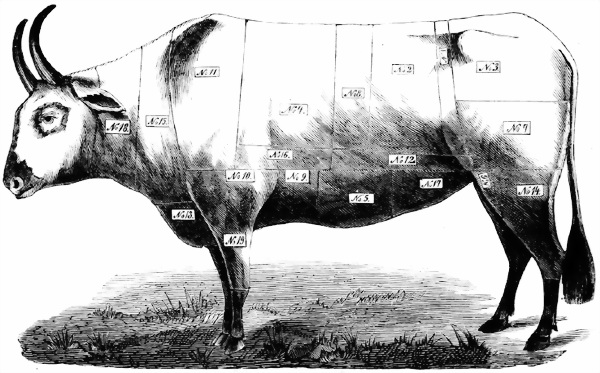
\includegraphics[width=\textwidth]{01.jpg}

Фигура 1-я изображает целого черкасского быка в натуральном его виде, а нумерованные подразделения означают места, где находится каждый из вышеупомянутых кусков.

Вот объяснение этой номенклатуры:

\noindent1. Английский филей. \\ 2. Толстый филей или вырезной. \\ 3. Огузок. \\ 4. Тонкий край. \\ 5. Завиток. \\ 6. Кострецы или подпашки. \\ 7. Середина бедра. \\ 8. Тонкий филей. \\ 9. Середина грудины. \\ 10. Середина лопатки. \\ 11. Толстый край. \\ 12. Подпашек \\ 13. Чолышко. \\ 14. Подбедерок. \\ 15. Оковалок. \\ 16. От края покромки. \\ 17. Бочок. \\ 18. Шея или зарез. \\ 19. Рулька.

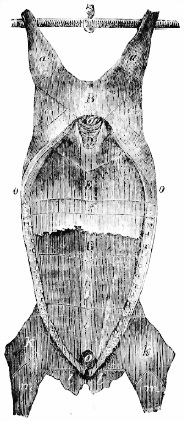
\includegraphics{02.jpg}

Фиг. 2-я есть туша, уже очищенная и развешенная на железных крючьях, при помощи палки, которую мясник продевает сквозь голяшки задних ног.

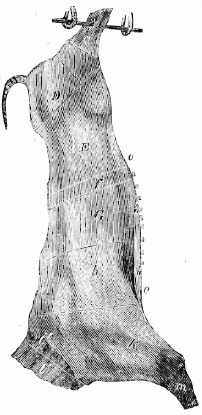
\includegraphics{03.jpg}

Фиг. 3-я есть та же туша, изображенная только боком, для большей ясности описания ее отдельных частей.

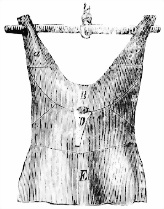
\includegraphics{04.jpg}

Фиг. 4-я представляет заднюю часть туши со стороны хребта.

Во всех этих фигурах одинаковые буквы показывают одни и те же куски туши, так что, рассматривая их в трех положениях, можно отлично заучить их отдельные формы.

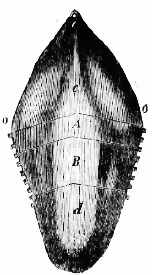
\includegraphics{05.jpg}

Фиг. 5-я изображает грудину с лицевой стороны.

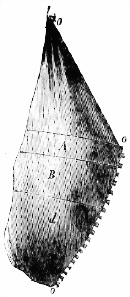
\includegraphics{06.jpg}

Фиг. 6-я изображает ее же сбоку, и здесь одинаковые буквы снова указывают на одинаковые куски или отдельные части грудины.

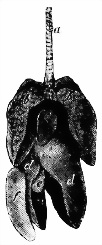
\includegraphics{07.jpg}

Фиг. 7-я изображает внутренности быка, т.~е. сердце, легкие, ливер, дыхательное горло, печенку и желчь.

Рассмотрев каждую фигуру по различным ее буквам, мы вполне и безошибочно ознакомимся со всеми частями туши.

Фиг. 2-я, 3-я и 4-я.

B. Нижняя подбрюшная часть или ссек, употребляемый преимущественно на жаркое,

а. а. Два подбедерка, идущие для бульона, если желаете иметь его наварнее.

C. C. Два подпашка, имеющие назначением заготовляться в прок в виде солонины.

D. Огузок, лучшая часть из всей туши, доставляющая отличный бульон; но и подаваемая отдельно в виде разварной говядины, или даже жаркого.

а. Часть дыхательного горла.

bb. Легкие, окружающие сердце; их употребляют в рубленом виде для пирогов, а иногда делают вкусное блюдо, называемое гаши (gachi).

с. Самое сердце.

dd. Гусак, или ливер; идет в начинку пирогов.

е. Печенка, из которой приготовляют род котлет.

ff. Желчный пузырь, материал для составления красок, а также употребляемый во множестве в аптеках.

Для лучшего узнавания этих отдельных частей бычачьей внутренности мы укажем и на различные их колера, как напр. сердце имеет темно-вишневый цвет и величиною бывает до 7 вершков, легкие~--- это мясистый, розово-фиолетовый кусок, гусак и печенка темно-вишневого цвета и две почки~--- тёмно-красные, глянцевитые куски мяса, облитые очень вкусным жиром. Почки употребляются под соусами и в суп-рассольник, а сало, их окружающее, идет во многие пирожные и в особенности в пудинги.

E. Филей, лакомая, по своей мягкости и сочности, часть туши. Филей разделяется на два сорта: английский и внутренний или вырезной. Места, ими занимаемые, указаны на фиг. 1 под №№ 1 и 2. Английский есть задняя часть филея, и его всегда почти употребляют на ростбиф, а вырезной доставляет настоящий бифстекс. Иные хозяйки берут филей для бульона, прельщаясь его мягким мясом в разварном виде; но это плохой расчет: филей стоит дорого, весу имеет очень много, потому что в нем заключается большая кость, а бульон от него никогда не бывает достаточно крепок, так как кость эта не имеет мозга.

F. Тонкий край, или I ребро, отсеченное в толщину всей туши. Из этого куска изготовляются котлеты, отделив мясо от костей, и его же употребляют на душеную говядину, так как вырезка его мягка, мясиста, хотя гораздо тверже филейной вырезки. Пользуясь неопытностью своих молодых хозяек, кухарки нередко заменяют этой вырезкой настоящую филейную и ставят ее на счет по той же дорогой цене. Филейная вырезка шире, мясистее и окружена большим количеством жира.

G. Грудина, т.~е. следующие за первым ребром четыре ребра, отрубаемые все вместе, чтоб составить этот кусок, употребляемый преимущественно для говяжьего битка.

H. Толстый край или оковалок, заключающий пять ребер и употребляемый для жирных щей.

I. Шея покупается для навара.

К. К. Две лопатки, идущие в развар для бульона.

М. М. Две голяшки, т.~е. оконечности передних ног; они жилисты, но дают превосходный, студенистый бульон, очень полезный для слабых людей; только должно старательнее снимать пену и давать долго кипеть: иначе бульон будет мутен и приобретет какой-то посторонний неприятный вкус.

L. L. Зарез, т.~е. самая оконечная часть шеи, жилистая, но годная для бульона.

оnо, оnо~--- покромки от края,~--- накожная мясистая оболочка, снятая с грудины и оканчивающаяся по направлению ребер; также идет в развар для бульона.

Р. (см. фиг. 8) изображает средину бедра, которую очень выгодно брать для бульона, так как в ней есть мозговая кость, а с тем вместе и мясо довольно нежно.

оооо. Показывает то место, или скорее ту впадину в туше, где находится грудина, которая изображена отдельно на фиг. 5 и 6-й.

С. (см. фиг. 5-ю) показывает бочок, или отдельную, верхнюю часть грудины, употребляемую для щей или борща.

А. Завиток есть та часть грудины, которая прилегает к двум первым ребрам и равномерно идет во щи или в борщ.

B. Собственно грудина, чрезвычайно жирная и хрящеватая часть мяса, состоящая из четырех ребер, и ее преимущественно употребляют, когда желают варить вкусный борщ.

d. Чолышко, нижняя часть грудины, мягкое и вкусное мясо, которое подают в виде разварной говядины с хреном.

Фиг. 7-я изображает внутренность быка, употребляемую в пищу, только тут не указаны рубец и селезенка, которая обвивается одним концом вокруг рубца, т.~е. большего беловатого куска внутренности желудка, а другим, т.~е. верхом, она находится в тесной связи с гусаком, или ливером. Селезенка имеет вид продолговатого, пестрого ремня мяситого цвета, с красноватыми и темными пятнами. Ее не употребляют в пищу люди; но она составляет часть, так называемой, кошачьей говядины, продаваемой гусачниками и кошатниками.

Мы уже сказали, что главная цель этого руководства~--- научить экономии молодых, неопытных хозяек. Для соблюдение полной экономии особенно при ограниченных средствах, необходимо входить в самые мелочи, уметь распоряжаться провизиею так, чтобы ничего не пропадало даром. Само собою разумеется, что этого нельзя требовать от прислуги, а потому было бы крайне неблагоразумно предоставлять эти заботы повару или кухарке. Поясним все вышесказанное примером: хозяйка небольшой семьи, например, из четырех человек, при закупке провизии на неделю (само собою разумеется, зимою), купила следующее: 12 фунтов ссеку, заднюю часть телятины (фунтов в 8 или 10), две телячьи головы, судака фунтов в пять и полдюжины телячьих ножек. Этою провизиею она всего выгоднее распорядится следующим образом: распределит говядину так, чтобы кости и часть мякоти шли на четыре супа (см. ниже: отд. V. Навары, бульоны, супы и пр.), а лучший мякотный кусок на котлеты для одного дня, тушеную говядину для другого обеда и клопфлейш для третьего; на четвертый день можно поджарить ножки с полуголяшкой и подать их под каким-нибудь соусом, употребив отвар из них на суп (см. королевский суп); из судака можно приготовить уху, русскую, немецкую и проч., а его подать под белым соусом с каперсами, с яйцами и~т.~д. Из телячьих же голов можно приготовить студень или из одной сварить суп, прибавив к ней полголяшки (если хотят иметь крепкий бульон) и подать ее на второе кушанье под соусом. Из задней части телятины выйдет жаркое на один день, из остатков которого на другой день, прибавив какой-нибудь отварной говядины, можно приготовить рагу, а из отрубленной голяшки и брюшной части, как было сказано выше, суп. Таким образом, предположив, что подобная провизия закуплена в субботу, хозяйка может из нее приготовить следующие обеды:

Воскресенье: 1-й суп из говядины (мы сказали, что из ссека можно приготовить суп), телячье жаркое с огурцами и пирог или пудинг.

Понедельник: 2-й суп из говядины, студень из головы, рагу.

Вторник: Уха, судак под скоромным соусом с картофелем и, если желают, кисель, блины или каша.

Среда: Суп из телячьих ножек с голяшкой, ножки с фасолью, зеленым горошком и~т.~д.

Четверг: 3-й суп из говядины, тушеная говядина с картофелем.

Пятница: Суп (наприм. рассольник) из голяшки и брюшной части телятины; котлеты с чечевицей, горошком, пюре из картофеля.

Суббота: 4-й суп из говядины, клопфлейш, каша\footnote{Само собою разумеется, что эти примечания относятся только до людей с небольшими средствами, имеющих простой стол}.

К этому мы считаем не лишним присовокупить еще следующие замечания, которые, как ни кажутся маловажны, однако же, в общей массе и в особенности для людей небогатых, имеют неоспоримое значение. Замечания эти следующие:

Перья и пух с домашних птиц и дичи следует копить и, перебрав в свободное время, сохранять в сухом месте. Ими можно набить подушки, перинки для детей и проч.

Выгребать уголья из печки и из-под плиты для самоваров.

Если бьют дома мелкий скот, то кровь сохранять. Ее подливают, для удобрения почвы, под фруктовые деревья.

Телячьи рубцы, хорошо вымыв в нескольких водах, высушить. Они употребляются при изготовлении швейцарских и голландских сыров, как сычуги, или лаба, о чем подробности в статье: <<Молочня>>.

Шкуры с телят, баранов и проч., тотчас по снятии, растянуть на палочки, высушить и отдать для выделки кож.

При каждой кухне хорошо держать двух или более поросят, которых можно кормить помоями, остатками кореньев, хлеба и~т.~д.; нужно только остерегаться, чтоб им не попадало мяса и остатков дичи.

Мыло для стирки лучше всего закупать по несколько брусьев, смотря по величине хозяйства, и сохранять его в сухом и теплом месте, потому что сухое мыло тверже и спорче. На один пуд белья выдавать 1 1/4 фун. мыла.

Обязанность каждой, разумеется, провинциальной и даже, просто-напросто, деревенской, хозяйки~--- входить во все эти мелочные подробности, надсматривать за порядком и чистотой, и стараться, чтоб малейшая безделица не пропадала даром. В столицах и больших городах все это немыслимо.

В этом руководстве, при описании кушаньев, т.~е. в большей части всех поваренных рецептов, принадлежащих г-же Авдеевой, назначена пропорция на три человека, т.~е. такая пропорция, при которой за обедом из трех или четырех блюд может быть вполне сыто семейство из трех человек. Эту пропорцию можно увеличить и уменьшить по желанию; так, например, на шесть человек удвоить, на девять утроить, на два взять 2/3 и~т.~д. Вполне соглашаясь с практичностью такого замечание покойной г-жи Авдеевой и сознавая возможность производить все расчисления блюд по сделанным ею здесь указаниям,~--- мы, занимаясь чисто практическими прибавлениями к книге г-жи Авдеевой, признали еще вполне целесообразным дополнить полезные эти заметки совершенно особенным и взятым с самой сути дела подробным расчетом обедов в 2–3 блюда, готовимых не из запасов, а из покупаемой провизии ежедневно на 10 человек. Цифра эта чрезвычайно удобна, как единица для расчислений различных обедов: вдвое меньшего числа потребителей, или, напротив, вдвое, втрое, в полтора раза большего. Расчисления г-жи N****, имевшей любезность передать в полное наше распоряжение свои <<домашние записки>>, помещены нами почти в конце книги, при распределении обедов или, так называемых, <<обеденных записок>> (меню). Эти расчисления доведены до последней степени точности и аккуратности, что поставляет мало-мальски смышленую хозяйку в удобную для нее возможность по этим примерам высчитывать все блюда этой книги с большею верностью и правильностью, чем ежели бы хозяйка эта руководствовалась совершенно готовыми расчетами провизии на каждое блюдо, предлагаемыми крайне наобум некоторыми нашими новомодными поваренными книгами.
